\usetikzlibrary{arrows}
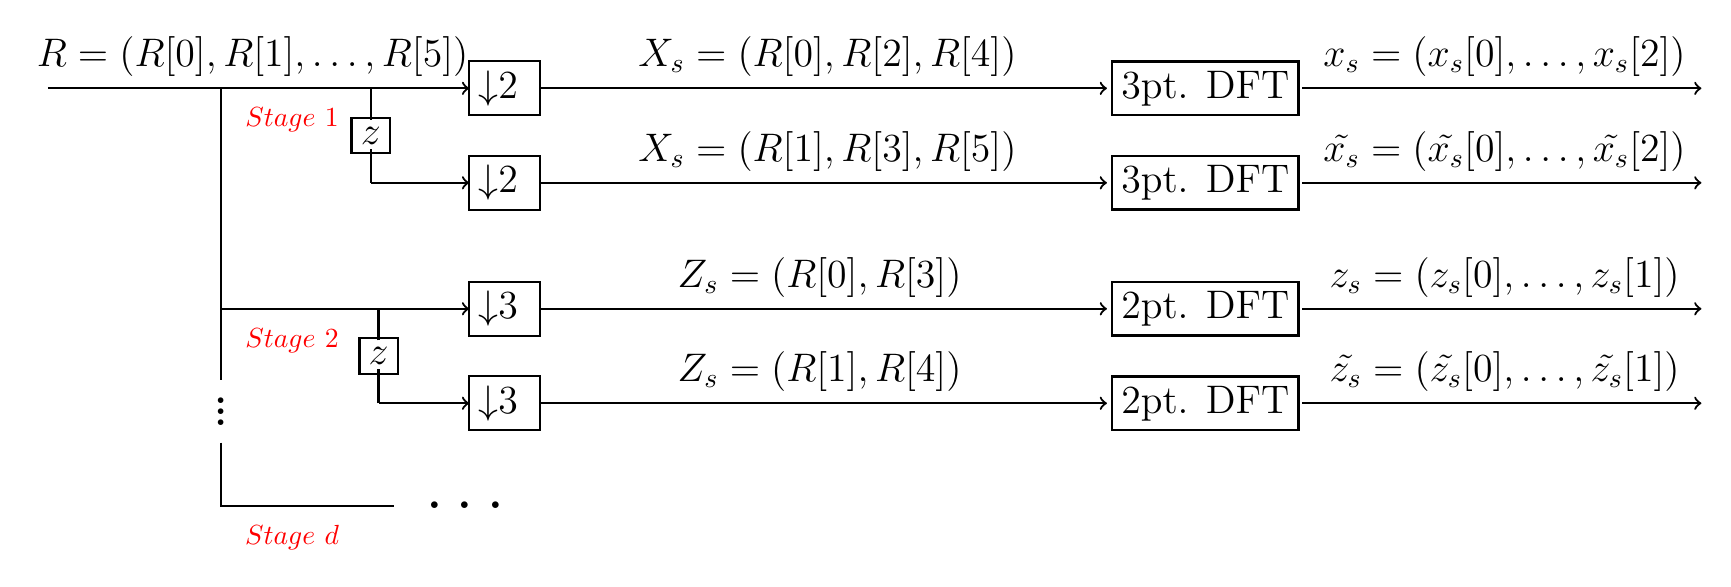
\begin{tikzpicture}

 % Downsampling blocks
\node[draw,align=center,thick] at (1.6,5.1) {\Large{$\mathbf{\downarrow} 3$} };
\node[draw,align=center,thick] at (1.6,6.3) {\Large{$\mathbf{\downarrow} 3$ }};

\node[draw,align=center,thick] at (1.6,7.9) {\Large{$\mathbf{\downarrow} 2$} };
\node[draw,align=center,thick] at (1.6,9.1) {\Large{$\mathbf{\downarrow} 2$ }};

%  Input lines to the down-sampling block
 \draw[->,thick] (0,5.1) -- (1.15,5.1);
 \draw[->,thick] (0,6.3) -- (1.15,6.3);
  
 \draw[->,thick] (-0.1,7.9) -- (1.15,7.9);
 \draw[->,thick] (-0.1,9.1) -- (1.15,9.1);

%  Delay blocks
\node[draw,align=center,thick] at (0,5.7) {\Large{$z$}};
\node[draw,align=center,thick] at (-0.1,8.5) {\Large{$z$}};

% paths connecting the delay blocks
 \draw[thick] (0,5.1) -- (0,5.53);
 \draw[thick] (0,5.9) -- (0,6.3);
 
 \draw[thick] (-0.1,7.9) -- (-0.1,8.33);
 \draw[thick] (-0.1,8.7) -- (-0.1,9.1);
 
% paths connecting the two stages   
 \draw[thick] (-0.1,9.1) -- (-2,9.1);
 \draw[thick] (0,6.3) -- (-2,6.3);
 \draw[thick] (-2,6.3) -- (-2,9.1);
  \draw[thick] (-4.2,9.1) -- (-2,9.1);
  \draw[thick] (-2,6.3) -- (-2,5.4);
  
  
  % DFT blocks
\node[draw,align=center,thick] at (10.5,5.1) {\Large{2pt. DFT}};
\node[draw,align=center,thick] at (10.5,6.3) {\Large{2pt. DFT}};

\node[draw,align=center,thick] at (10.5,7.9) {\Large{3pt. DFT}};
\node[draw,align=center,thick] at (10.5,9.1) {\Large{3pt. DFT}};

% Connectors
 \draw[->,thick] (2.05,9.1) -- (9.25,9.1);
 \draw[->,thick] (2.05,7.9) -- (9.25,7.9);
  
 \draw[->,thick] (2.05,6.3) -- (9.25,6.3);
 \draw[->,thick] (2.05,5.1) -- (9.25,5.1);

 \draw[->,thick] (11.73,9.1) -- (16.8,9.1);
 \draw[->,thick] (11.73,7.9) -- (16.8,7.9);
 
 \draw[->,thick] (11.73,6.3) -- (16.8,6.3);
 \draw[->,thick] (11.73,5.1) -- (16.8,5.1);
 
 
  % Labels
  \node[draw=none,align=center] at (-1.6,9.5) {\Large{$R=(R[0],R[1], \ldots, R[5])$}};
  
  \node[draw=none,align=center] at (5.7,9.5) {\Large{$X_{s}=(R[0],R[2],R[4])$}};
  \node[draw=none,align=center] at (5.7,8.3) {\Large{$X_{s}=(R[1],R[3],R[5])$}};
  \node[draw=none,align=center] at (5.6,6.7) {\Large{$Z_{s}=(R[0],R[3])$}};
  \node[draw=none,align=center] at (5.6,5.5) {\Large{$Z_{s}=(R[1],R[4])$}};
  
  \node[draw=none,align=center] at (14.3,9.5) {\Large{$x_{s}=(x_{s}[0],\ldots,x_{s}[2])$}};
  \node[draw=none,align=center] at (14.3,8.3) {\Large{$\tilde{x_{s}}=(\tilde{x_{s}}[0],\ldots,\tilde{x_{s}}[2])$}};
  \node[draw=none,align=center] at (14.3,6.7) {\Large{$z_{s}=(z_{s}[0],\ldots,z_{s}[1])$}};
  \node[draw=none,align=center] at (14.3,5.5) {\Large{$\tilde{z_{s}}=(\tilde{z_{s}}[0],\ldots,\tilde{z_{s}}[1])$}};
  
  \node [draw=none] at (-2,5.1) {\Huge${\vdots}$} ;
  
   \node[draw=none,align=center] at (-1.1,8.7) {\color{red}$Stage ~1$};
  \node[draw=none,align=center] at (-1.1,5.9) {\color{red}$Stage ~2$};
   \node[draw=none,align=center] at (-1.1,3.4) {\color{red}$Stage ~d$};
\draw [thick](-2,4.6) -- (-2,3.8) -- (0.2,3.8) ;
 \node[draw=none,align=center] at (1.1,3.8) {\Huge${\ldots}$};
\end{tikzpicture}